\documentclass{article}


\usepackage{amsmath} % math stuff
\usepackage{amssymb} % math stuff
\usepackage{array} % equations and stuff
\usepackage{bm} % bold math
%\usepackage{caption} % suppressed table numbering; incompatible with revtex, and longtable, I think
\usepackage{comment} % comment environment
%\usepackage{enumitem} % customization of enumeration, itemize, and description
\usepackage[T1]{fontenc} % font encoding for special characters, must also use scalable font package
\usepackage[margin=0.8in]{geometry} % paper sizes and margins (but be careful not to mess up pre-defined pages)
\usepackage{graphicx} % for graphics
%\usepackage{helvet} % default font is the helvetica postscript font
\usepackage{lipsum} % lorem ipsum filler text
\usepackage{lmodern} % scalable font?
\usepackage{longtable} % multi-page tables
\usepackage{mathrsfs} % math script font
\usepackage{mhchem} % easier chemical formula
\usepackage{microtype} % allows disabling of ligatures
%\usepackage{newcent} % new century schoolbook font
\usepackage{nicefrac}
\usepackage{parskip} % removes paragraph indentation, and adjusts paragraph skip, as well as list items
%\usepackage{setspace} % adjust text spacing and indents
\usepackage{siunitx} % decimal alignment
\usepackage{subfigure} % divided figures
%\usepackage{tabu} % extra table options
\usepackage{textcomp} % symbols
\usepackage{threeparttablex} % better footnotes with longtable
\usepackage{titling} % title placement
\usepackage{ulem} % strikethrough text
%\usepackage{url} % superceded by hyperref
\usepackage{verbatim} % verbatim environment
\usepackage{xcolor} % colors and color boxes
\usepackage{xspace} % commands that don't eat up white space
\usepackage{hyperref} % links and page setup; should always come last

\hypersetup{
	bookmarks=true,
	colorlinks=true,
	citecolor=blue,
	linkcolor=blue,
	urlcolor=blue,
	pdfstartview={XYZ null null 1.0} % default open view is 100%
}

\DisableLigatures[f]{encoding = *, family = * } % disable ff, fi, fl ligatures, without f option, it also disables -- = endash
\renewcommand{\arraystretch}{1} % extra vertical space in tables

\begin{document}

\pagestyle{empty} % don't number pages

% custom title
\begin{center}
{\LARGE Express Riddler}

\vspace{0.15in}

{\Large 29 May 2020}
\end{center}


\section*{Riddle:}

While spending more time at home in recent weeks, I've had the chance to revisit one of my favorite video games from recent years — The Legend of Zelda: Breath of the Wild.
Within the game, there are hundreds of hidden ``Korok Seeds'', which I'm having an increasingly difficult time finding.

Fortunately, there's a special mask you can acquire in the game that makes a sound any time you're within a certain distance of a Korok Seed.
While playing, I marked nine distinct locations on the game map, forming the 3-by-3 grid shown below:
\begin{center}
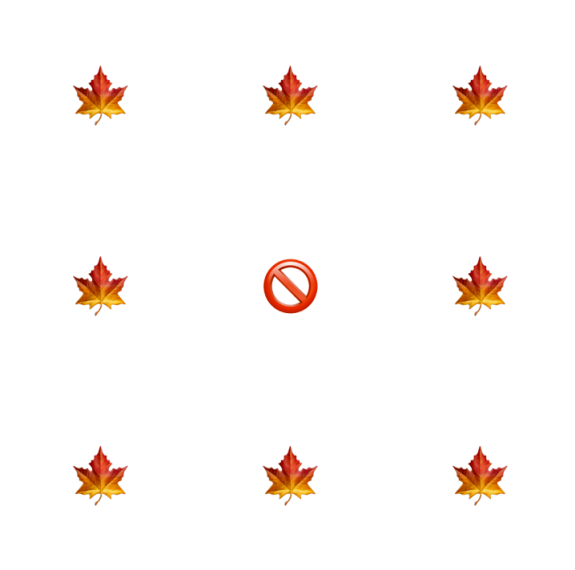
\includegraphics[width=3in]{seed_map.png}
\end{center}
Each leaf symbol is within range of a Korok Seed, while the point in the middle is \textit{not} within range of a Korok Seed.
Given this arrangement, what is the minimum possible number of Korok Seeds I could have detected?

\section*{Solution:}

Surprisingly, it is possible for this arrangement to occur from only
\fcolorbox{red}{white}{\bf two seeds}\,.
The only condition necessary for a solution is that the distance from the center point to either seed is greater than the distance from any other point to the nearest seed, regardless of the particular detection range.
I will illustrate a solution with the diagram below:

\vspace{0.1in}
\begin{center}
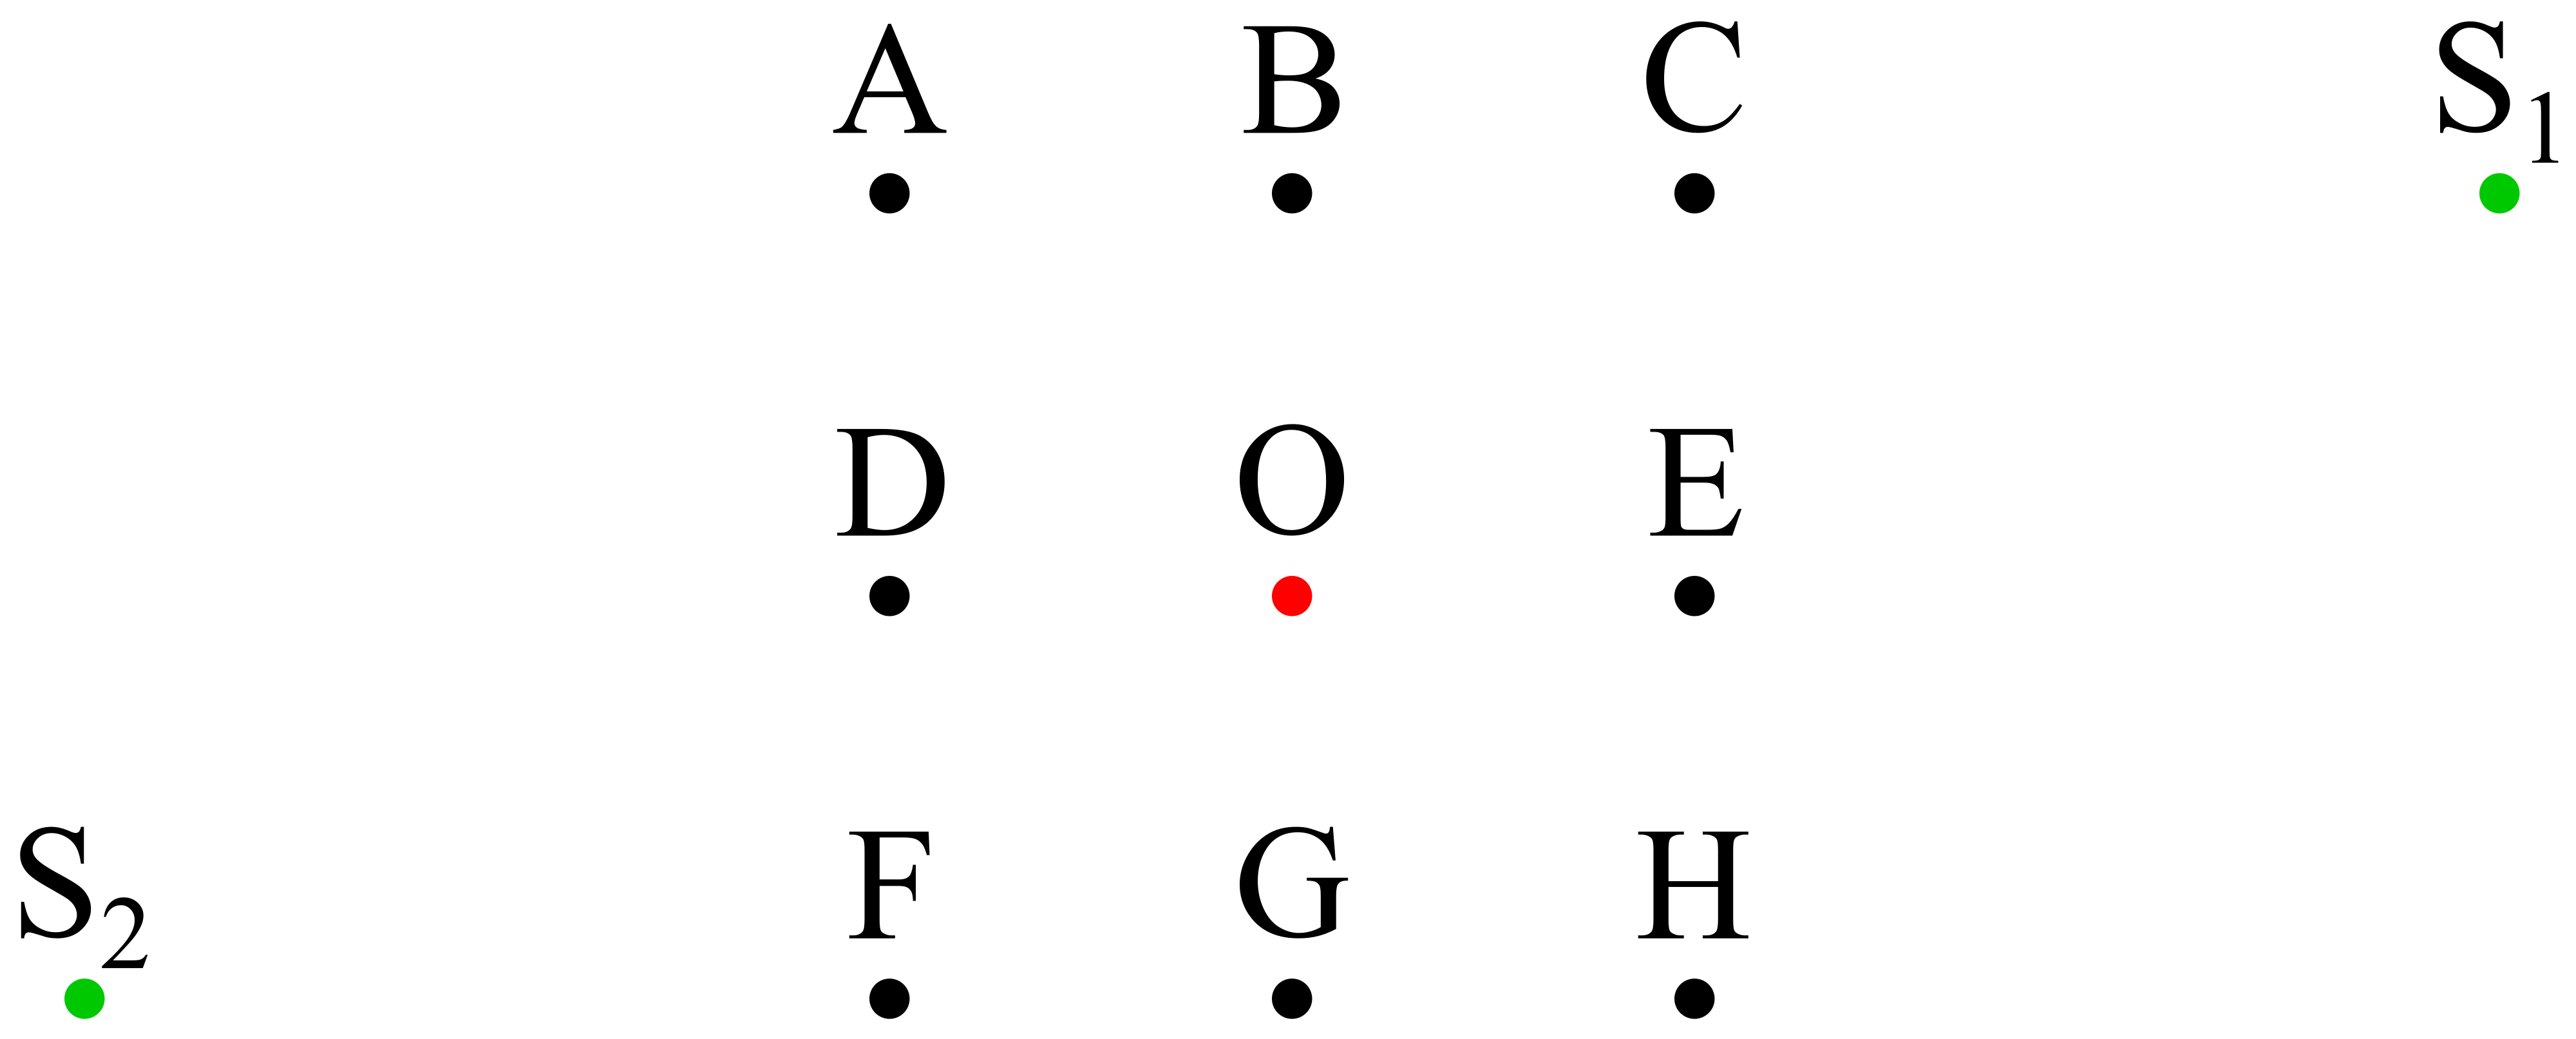
\includegraphics[width=4.8in]{seed_diagram.png}
\end{center}
\vspace{0.1in}

I have labeled each of the detection points A--H, the non-detection point O, and the two seed points $\mathrm{S}_{1}$ and $\mathrm{S}_{2}$.
To quantify the problem, suppose that O is at the origin, and the surrounding detection points are located at $(-1,1)$, $(0,1)$, $(1,1)$, etc.
Also suppose $\mathrm{S}_{1}$ is located at $(3,1)$ and $\mathrm{S}_{2}$ at $(-3,-1)$.
Then, we have $\overline{\mathrm{BS}_{1}}=3$, $\overline{\mathrm{CS}_{1}}=2$, $\overline{\mathrm{ES}_{1}}=\sqrt{5}$, $\overline{\mathrm{HS}_{1}}=\sqrt{8}$, and $\overline{\mathrm{OS}_{1}}=\sqrt{10}$.
The situation is the same for $\mathrm{S}_{2}$ by symmetry.
Because the distance from the origin to the seeds is larger than the other distances ($\sqrt{10}>3>\sqrt{8}>\sqrt{5}>2$), the necessary condition is met.
Thus as long as the detection range is larger than 3 times the unit distance, but less than $\sqrt{10}$ times, we can construct the above grid. 



\end{document}